\documentclass{article}
\title{What Factors Contribute to a Starbuck’s Star Rating on Yelp?}
\date{5/6/2016}
\author{Youyou Tian and Alice Yang}
\usepackage{multicol}
\usepackage[margin=.75in]{geometry}
\usepackage{enumitem}
\usepackage{graphicx}
\usepackage{caption}

\newenvironment{Figure}
  {\par\medskip\noindent\minipage{\linewidth}}
  {\endminipage\par\medskip}

\begin{document}
\maketitle{}
\begin{multicols}{2}

\section{Introduction}

	Chain restaurants try to standardize the quality of service in each of their franchises. Assuming the service quality stays constant, how much of the success of a restaurant, judged by the average star rating on yelp, is dependent on its location or services?

\section{Data and Methods}

	In order to answer the above question, we have used the Yelp Dataset from the Yelp Dataset Challenge 2016 and the US Census dataset from 2010 - 2014. The Yelp Dataset is composed of business data from US cities Pittsburgh, Charlotte, Urbana-Champaign, Phoenix, Las Vegas, and Madison. The Yelp dataset itself contained information on the restaurant’s location as well as amenities. In particular, we were interested in the Starbucks coffeehouse chain because we knew there would be a lot of data points from the dataset, being a global corporation. The US Census contained detailed information about each geographical region. The predictors we picked were based on what we had assumed would affect average Yelp star rating. These predictors included information based on the geographical location of the Starbucks as well as any services provided. Our initial list consisted of: 

\begin{itemize}[noitemsep,topsep=8pt,parsep=0pt,partopsep=0pt]
	\item Average rating
	\item Total population of the area
	\item Percentage of the caucasian population
	\item Average household income
	\item Average household size
	\item Wifi availability
	\item Wheelchair accessible
	\item Price range (1-5 scale)
	\item Payment by credit card
	\item Outdoor seating availability
	\item Lot parking presence
	\item Street parking presence
\end{itemize}

	To obtain the information needed, we first parsed the Yelp dataset from a JSON format using Starbucks, filtering by Starbucks businesses. Next, we then used Python to query the US Census API based on the zip code provided by each Starbucks to obtain more geographical location. 

\section{Results}

	From the data we have collected, we then used R to run various methods. For all the supervised methods we tried, we separated our data randomly in half to form a training set and a test set. 

\begin{Figure}
\centering
   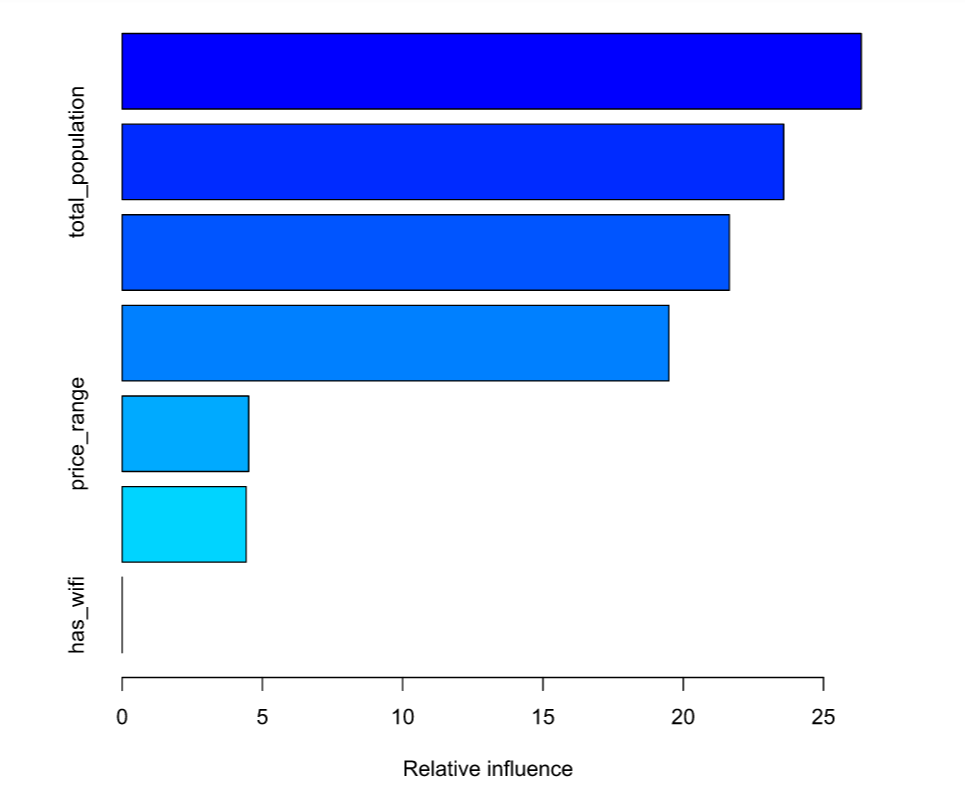
\includegraphics[width=\linewidth]{boostingChart}
	\captionof{figure}{Boosting chart}\label{fig:boost}
\end{Figure}

	First, we created a regression tree and then applied boosting (Figure \ref{fig:boost}). From the boosting data, we were able to narrow down the list of predictors to the following list:

\begin{itemize}[noitemsep,topsep=8pt,parsep=0pt,partopsep=0pt]
	\item Average rating
	\item Total population of the area
	\item Percentage of the caucasian population
	\item Average household income
	\item Average household size
	\item Wifi availability
	\item Wheelchair accessible
	\item Price range (1-5 scale)
\end{itemize}

We removed the following predictors because we saw that every Starbucks had these features, so it made no impact on any model.

\begin{itemize}[noitemsep,topsep=8pt,parsep=0pt,partopsep=0pt]
\item Payment by credit card
\item Outdoor seating availability
\item Lot parking presence
\item Street parking presence
\end{itemize}

\begin{Figure}
\centering
   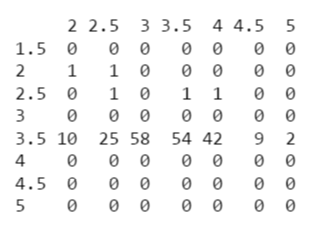
\includegraphics[width=\linewidth]{confusionMatrixLda}
	\captionof{figure}{Confusion matrix of LDA results}\label{fig:confmat}
\end{Figure}

Once we had an idea on the type of predictors to try, we then used best subset to further narrow down our set of predictors. We chose to use best subset because we only had eight predictors after the initial boosting. We were then able to further narrow down our predictors to being: percentage of the caucasian population within the given zip code, the price range of Starbucks, and if there is wifi available. From the narrowed set of predictors, we ran LDA and received a test error rate of about 27\%. This could mean that there is some relation between the percentage of the caucasian population and star ratings. 

Interestingly, the confusion matrix (Figure \ref{fig:confmat}) after running LDA showed that the model almost consistently picked 3.5 as the average star rating of a given Starbucks restaurant.

\begin{Figure}
\centering
   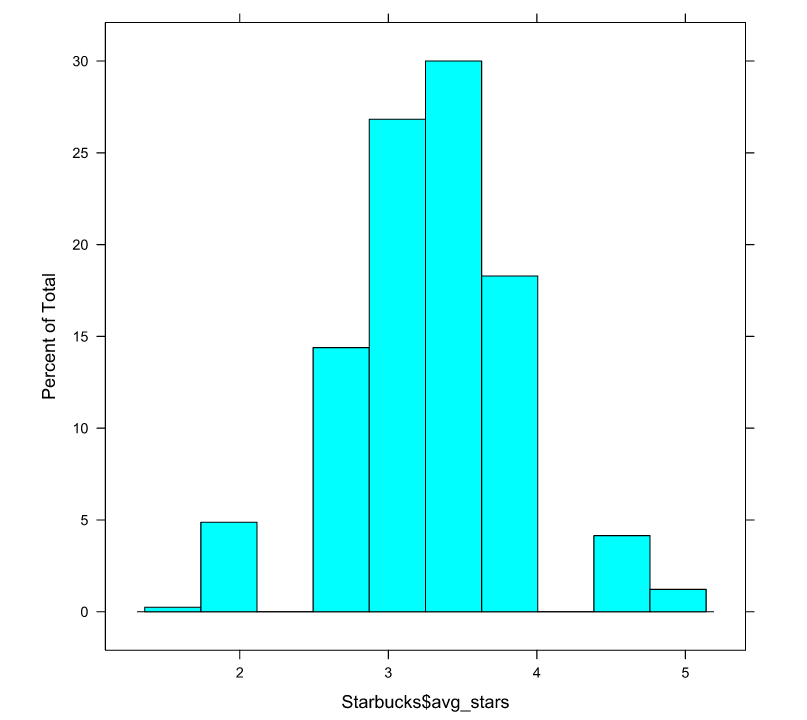
\includegraphics[width=\linewidth]{avgstars}
	\captionof{figure}{Histogram of dataset distribution of the average star rating}\label{fig:hist}
\end{Figure}

We checked the distribution of the average stars from the dataset and saw that the majority of the ratings were clustered around 3 - 4 stars, with the mode being 3.5 stars (Figure \ref{fig:hist}). Though the model always picked 3.5 stars, the low test error rate makes sense because indeed the majority of the data had fallen within that range. 

We had also ran PCA on the first narrowed list of predictors picked from bagging to see if there were any interesting properties of the data. 

\begin{Figure}
\centering
   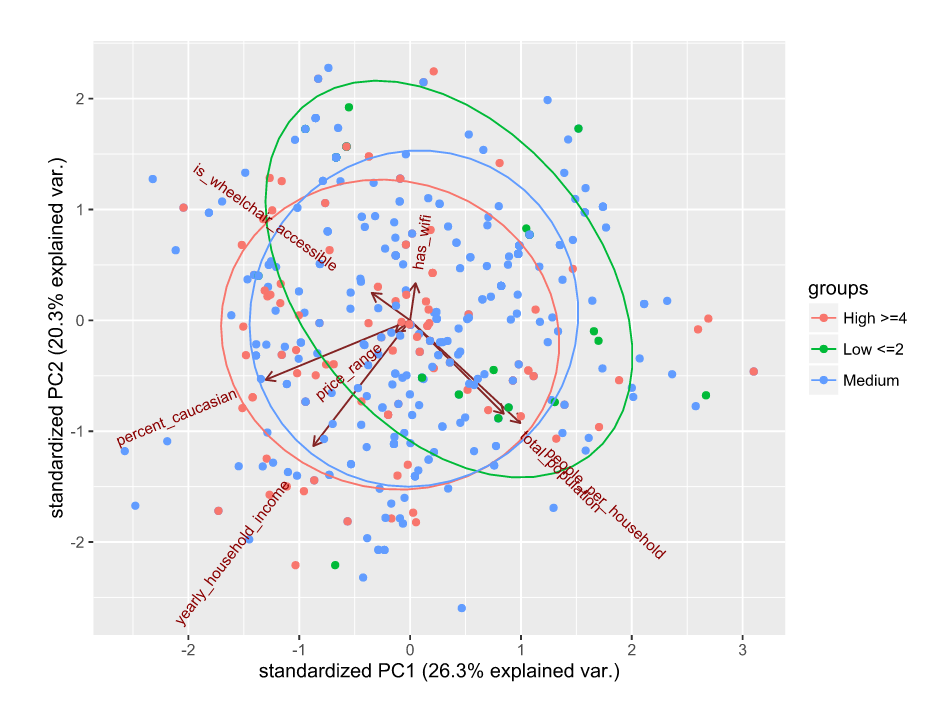
\includegraphics[width=\linewidth]{pc12}
	\captionof{figure}{PCR on the 1st and 2nd principal components}\label{fig:pc12}
\end{Figure}

Matching what we noticed from LDA, the first and second principal components (Figure \ref{fig:pc12}) show that the lower average star ratings tend to be opposite the vectors representing the percentage of the caucasian population and yearly household income. Additionally, the higher ratings tend more towards the mentioned vectors. Middle ratings were evenly spread across all vectors. What constitutes as a “low” rating versus a “high” rating was determined from the ratings distribution from Figure  \ref{fig:pcavgstars}. There was a clear break between the ratings at and below 2 stars and the ratings at or above 4 stars. The break lead us to make the judgement to categorize the rankings as discussed above. 

We also took a look at the other principal components because though the first and second principal component described 26.3\% and 20.3\% of the variance respectively, the third and fourth principal components also described a large percentage of the variance as well (16.6/% and 14/% of the variance respectively). 

\begin{Figure}
\centering
   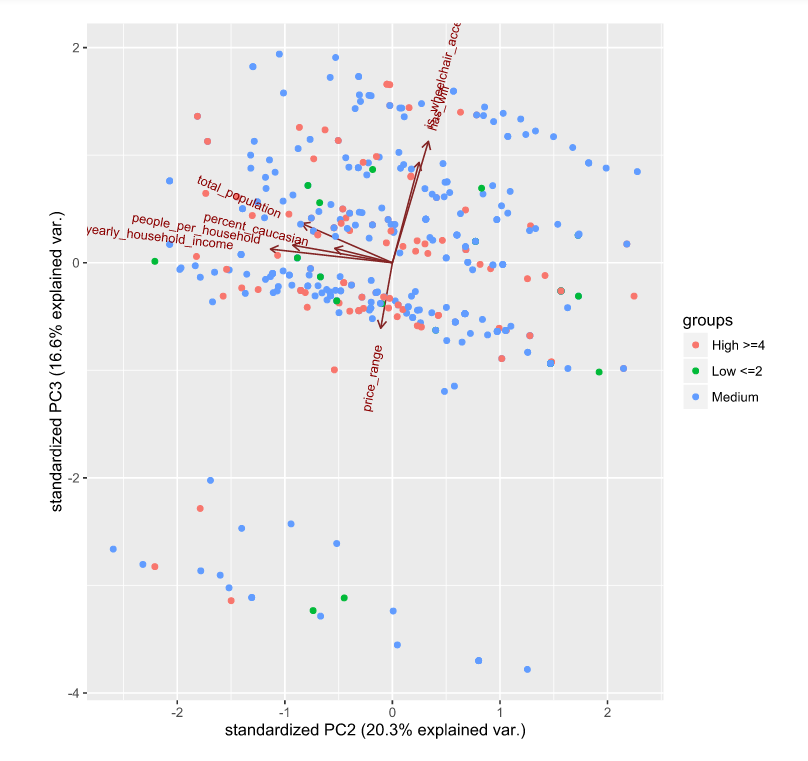
\includegraphics[width=\linewidth]{pc23}
	\captionof{figure}{PCR on the 2nd and 3rd principal components}\label{fig:pc23}
\end{Figure}

Comparing the second and third principal components (Figure \ref{fig:pc23}), we notice interesting strips that run parallel to the price range vector. From the predictors chosen, it is hard to discern clear rating groupings. However, we could make an assumption that the effect is only to do with price range. The other vectors pulling are whether the location is wheelchair accessible or has wifi, which were both recorded as boolean values. It could be possible some combination of the 3 eigenvectors have are the reason for such a pattern. 

Finally, we take a look at the third and fourth principal components (Figure \ref{fig:pc34}). There are clear groupings between the data that again seem to be split along price range. It is possible that PCR is hinting we are missing predictors that could explain the groupings shown.

\begin{Figure}
\centering
   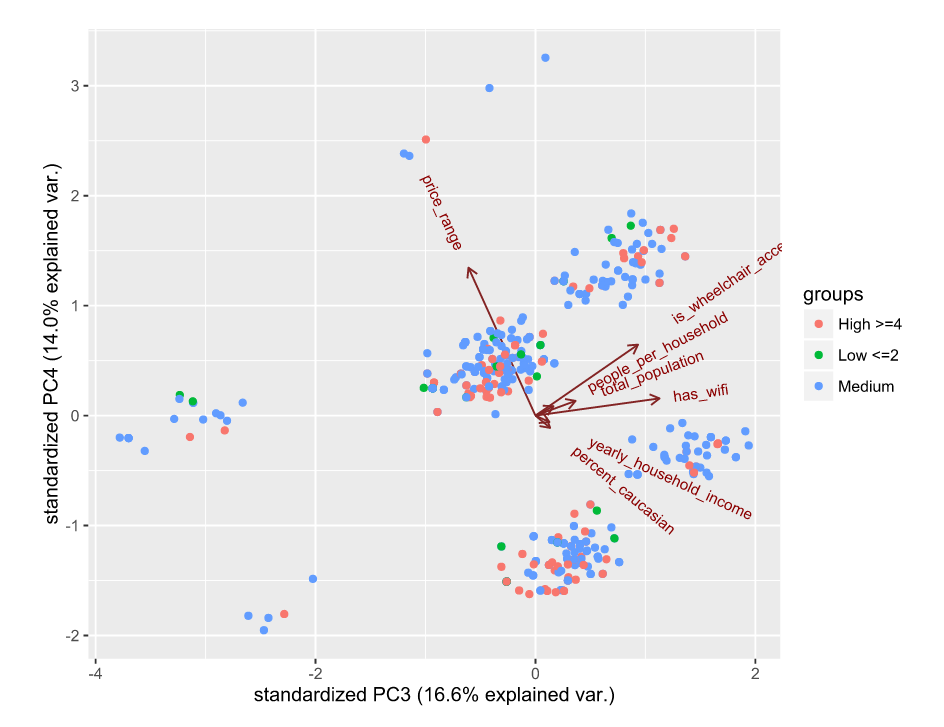
\includegraphics[width=\linewidth]{pc34}
	\captionof{figure}{PCR on the 3rd and 4th principal components}\label{fig:pc34}
\end{Figure}

\section{Conclusion and Future Work}

Based on our results from LDA and PCR, we can conclude that the price range and the percent of caucasians are correlated with the Yelp star ratings. We realize that the effect of the percent caucasians may be die to the limited city choices given from the yelp data. The majority of our Starbucks data came from Pittsburgh, which does have a high caucasian population, about 66\% in 2010 \footnote{\label{footnote1} "Population Estimates, July 1, 2015, (V2015)." Pittsburgh City Pennsylvania QuickFacts from the US Census Bureau. Web. 06 May 2016. <http://www.census.gov/quickfacts/table/PST045215/4261000\#flag-js-X>}. As such,our models may only represent Pittsburgh Starbucks and not the chain nationally. In all, it is possible to confirm the Starbucks stereotype that it is a chain advertized more towards the rich caucasian populace. 

There is still much more that we wish to analyze with the data. First, we realize that we had a limited amount of predictors for this analysis. We would like to get more predictors, such as general climate conditions of the area, the density of competing restaurants within the area and business hours of the restaurant. We can also look towards natural language processing to include reviews as additional predictors as well. Finally, we would like to expand past the Starbucks chain and look at a wider range of large chains, such as Dunkin’  Donuts or McDonalds and see if our model can be used to predict other Yelp ratings.

\section{Sources}

\begin{enumerate}[noitemsep,topsep=8pt,parsep=0pt,partopsep=0pt]
\item Yelp dataset 2016
\item US Census dataset 2010 - 2014
\end{enumerate}

\end{multicols}

\end{document}